\documentclass[landscape,final,a0paper,fontscale=0.285]{baposter}

\usepackage{calc}
\usepackage{caption}
\usepackage{graphicx}
\usepackage{amsmath}
\usepackage{amssymb}
\usepackage{relsize}
\usepackage{multirow}
\usepackage{rotating}
\usepackage{bm}
\usepackage{url}

\usepackage{graphicx}
\usepackage{multicol}

\usepackage{palatino}

\usetikzlibrary{calc}

%%%%%%%%%%%%%%%%%%%%%%%%%%%%%%%%%%%%%%%%%%%%%%%%%%%%%%%%%%%%%%%%%%%%%%%%%%%%%%%%
% Multicol Settings
%%%%%%%%%%%%%%%%%%%%%%%%%%%%%%%%%%%%%%%%%%%%%%%%%%%%%%%%%%%%%%%%%%%%%%%%%%%%%%%%
\setlength{\columnsep}{1.5em}
\setlength{\columnseprule}{0mm}

%%%%%%%%%%%%%%%%%%%%%%%%%%%%%%%%%%%%%%%%%%%%%%%%%%%%%%%%%%%%%%%%%%%%%%%%%%%%%%%%
% Save space in lists. Use this after the opening of the list
%%%%%%%%%%%%%%%%%%%%%%%%%%%%%%%%%%%%%%%%%%%%%%%%%%%%%%%%%%%%%%%%%%%%%%%%%%%%%%%%
\newcommand{\compresslist}{%
\setlength{\itemsep}{1pt}%
\setlength{\parskip}{0pt}%
\setlength{\parsep}{0pt}%
}

%%%%%%%%%%%%%%%%%%%%%%%%%%%%%%%%%%%%%%%%%%%%%%%%%%%%%%%%%%%%%%%%%%%%%%%%%%%%%%
%%% Begin of Document
%%%%%%%%%%%%%%%%%%%%%%%%%%%%%%%%%%%%%%%%%%%%%%%%%%%%%%%%%%%%%%%%%%%%%%%%%%%%%%

\begin{document}

%%%%%%%%%%%%%%%%%%%%%%%%%%%%%%%%%%%%%%%%%%%%%%%%%%%%%%%%%%%%%%%%%%%%%%%%%%%%%%
%%% Here starts the poster
%%%---------------------------------------------------------------------------
%%% Format it to your taste with the options
%%%%%%%%%%%%%%%%%%%%%%%%%%%%%%%%%%%%%%%%%%%%%%%%%%%%%%%%%%%%%%%%%%%%%%%%%%%%%%
% Define some colors

%\definecolor{lightblue}{cmyk}{0.83,0.24,0,0.12}
\definecolor{lightblue}{rgb}{0.145,0.6666,1}

%%
\begin{poster}%
  % Poster Options
  {
  % Show grid to help with alignment
  grid=false,
  % Column spacing
  colspacing=1em,
  % Color style
  bgColorOne=white,
  bgColorTwo=white,
  borderColor=lightblue,
  headerColorOne=black,
  headerColorTwo=lightblue,
  headerFontColor=white,
  boxColorOne=white,
  boxColorTwo=lightblue,
  % Format of textbox
  textborder=roundedleft,
  % Format of text header
  eyecatcher=true,
  headerborder=closed,
  headerheight=0.1\textheight,
%  textfont=\sc, An example of changing the text font
  headershape=roundedright,
  headershade=shadelr,
  headerfont=\Large\bf\textsc, %Sans Serif
  textfont={\setlength{\parindent}{1.5em}},
  boxshade=plain,
%  background=shade-tb,
  background=plain,
  linewidth=2pt
  }
  % Eye Catcher
  {
\includegraphics[height=7em]{figures/ungLogo.jpg}} 
  % Title
  {\bf\textsc{A Comparative Study of Particle Identification Techniques}\vspace{0.25em}}
  % Authors
  {
    Cody Brown, Mireya Flores, Kalanie Wilson, Dr. Nathan Harrison \\
    \vspace{2mm}
    Department of Physics, The University of North Georgia, Oakwood, GA 30566
  }

%%%%%%%%%%%%%%%%%%%%%%%%%%%%%%%%%%%%%%%%%%%%%%%%%%%%%%%%%%%%%%%%%%%%%%%%%%%%%%
%%% Now define the boxes that make up the poster
%%%---------------------------------------------------------------------------
%%% Each box has a name and can be placed absolutely or relatively.
%%% The only inconvenience is that you can only specify a relative position 
%%% towards an already declared box. So if you have a box attached to the 
%%% bottom, one to the top and a third one which should be in between, you 
%%% have to specify the top and bottom boxes before you specify the middle 
%%% box.
%%%%%%%%%%%%%%%%%%%%%%%%%%%%%%%%%%%%%%%%%%%%%%%%%%%%%%%%%%%%%%%%%%%%%%%%%%%%%%

%%%%%%%%%%%%%%%%%%%%%%%%%%%%%%%%%%%%%%%%%%%%%%%%%%%%%%%%%%%%%%%%%%%%%%%%%%%%%%
  \headerbox{Abstract}{name=abstract,column=0,row=0,span=2}{
%%%%%%%%%%%%%%%%%%%%%%%%%%%%%%%%%%%%%%%%%%%%%%%%%%%%%%%%%%%%%%%%%%%%%%%%%%%%%%
\noindent{
Typical high energy experiments in particle physics involve collisions between different subatomic particles.
The goal of these collisions is to force the particles to break apart into their constituents, thus giving insights into the structure of matter at the smallest known scales.
In order to ``see'' the products of a collision, complex particle detector systems are built around the collision point such that the final state particles travel through the different detectors leaving behind some measurable signal.
From these detector responses it is possible to deduce a particle's kinematics and type.
This particle identification (PID) process is essential for any high-level analysis, however, due to effects such as detector resolution and inefficiencies it can be highly non-trivial.
This work is a comparative study of the following PID techniques: (1) the traditional cut-based approach, (2) a machine-learning approach, and (3) a probability-based approach.
}
}

%%%%%%%%%%%%%%%%%%%%%%%%%%%%%%%%%%%%%%%%%%%%%%%%%%%%%%%%%%%%%%%%%%%%%%%%%%%%%%
  \headerbox{Introduction}{name=introduction,column=0,below=abstract,span=2}{
%%%%%%%%%%%%%%%%%%%%%%%%%%%%%%%%%%%%%%%%%%%%%%%%%%%%%%%%%%%%%%%%%%%%%%%%%%%%%%
\noindent{
This study used a GEANT $[1]$ based simulation of the CLAS detector located at Jefferson National Laboratory $[2]$ with over 600k generated particle events with the goal of sorting the particles by type based on six detector responses (p, $\theta$, $\beta$, \v{C}erenkov counts, and two calorimeter energies).
The 3 aforementioned techniques were tested and compared based of their efficiency and purity, table \ref{tab:pidSamplesTable} shows a hypothetical result.
}
%
\begin{center}
\begin{minipage}[c]{0.44\linewidth}
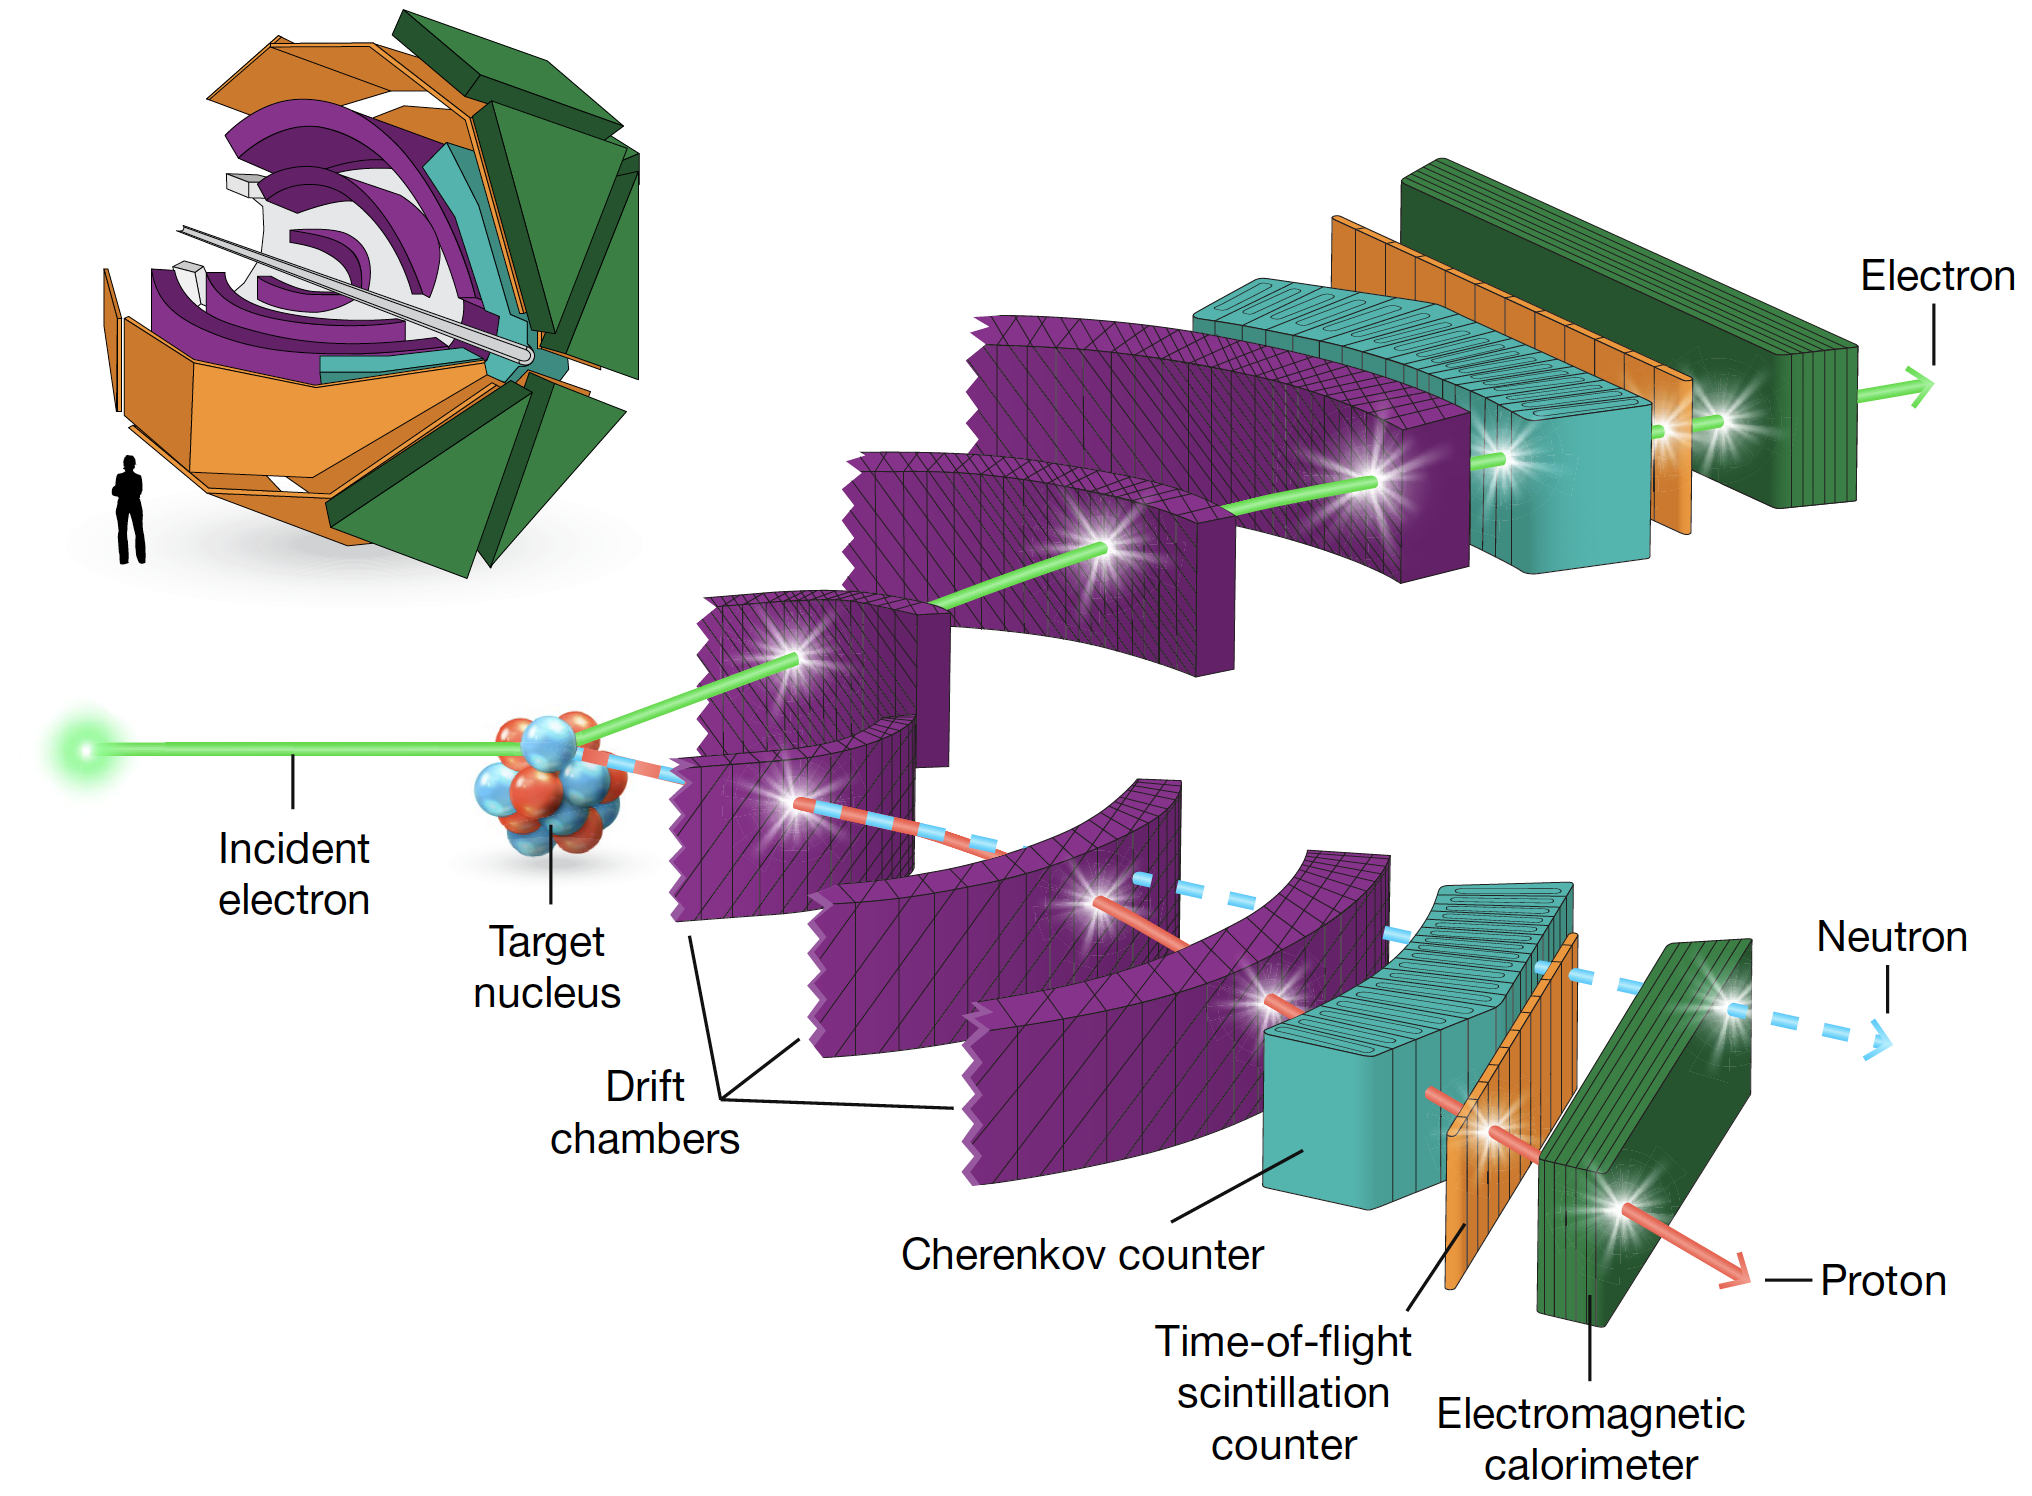
\includegraphics[width=\linewidth]{figures/clas.png}
\end{minipage}
\hfill
\begin{minipage}[c]{0.54\linewidth}
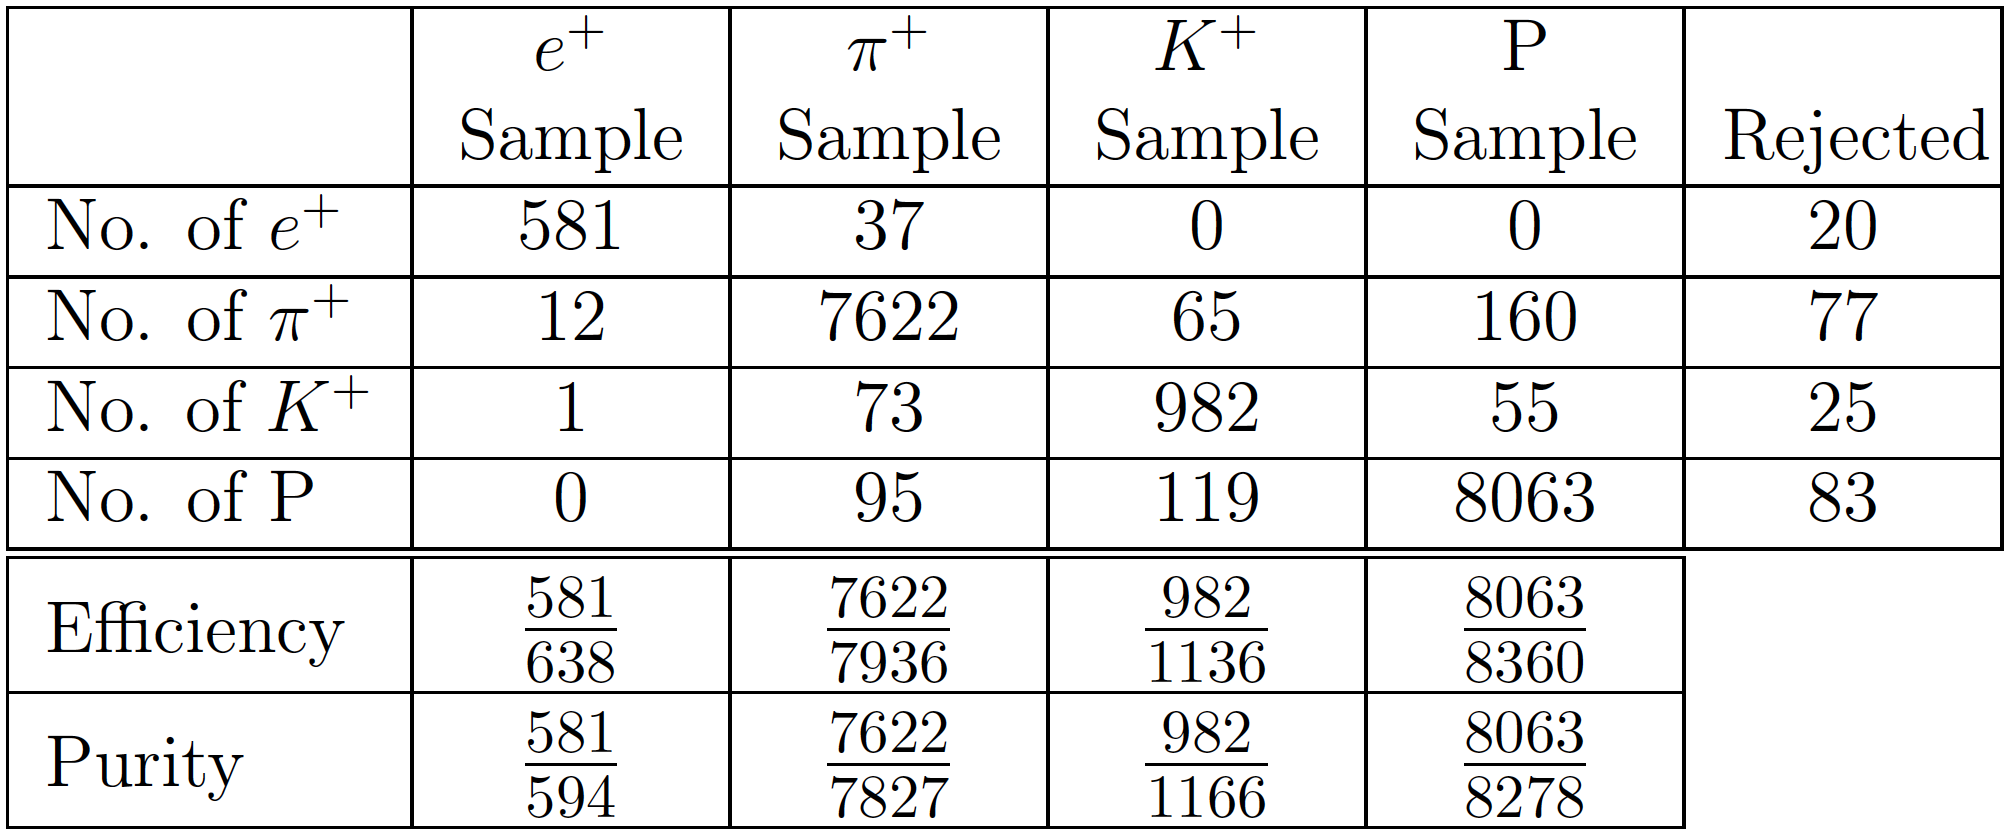
\includegraphics[width=\linewidth]{figures/pidSamplesTable.png}
\vspace{-6mm}
\captionof{table}{(Above) Hypothetical efficiency and purity for the four particle samples.}
\label{tab:pidSamplesTable}
\vspace{-2mm}
\captionof{figure}{(Left) The CLAS detector $[2]$ $[3]$. \hfill \protect\phantom{A}}
\label{fig:clas}
\end{minipage}
\end{center}
}

%%%%%%%%%%%%%%%%%%%%%%%%%%%%%%%%%%%%%%%%%%%%%%%%%%%%%%%%%%%%%%%%%%%%%%%%%%%%%%
  \headerbox{Methods}{name=methods,column=2,row=0,span=2}{
%%%%%%%%%%%%%%%%%%%%%%%%%%%%%%%%%%%%%%%%%%%%%%%%%%%%%%%%%%%%%%%%%%%%%%%%%%%%%%
The first PID method is the traditional cut-based approach.
As shown in figure~\ref{fig:bvp_all}, upper and lower velocity ($\beta$) limits are defined based on the relativistic relationship between momentum, mass, and velocity.
%
\begin{center}
\begin{minipage}[c]{0.44\linewidth}
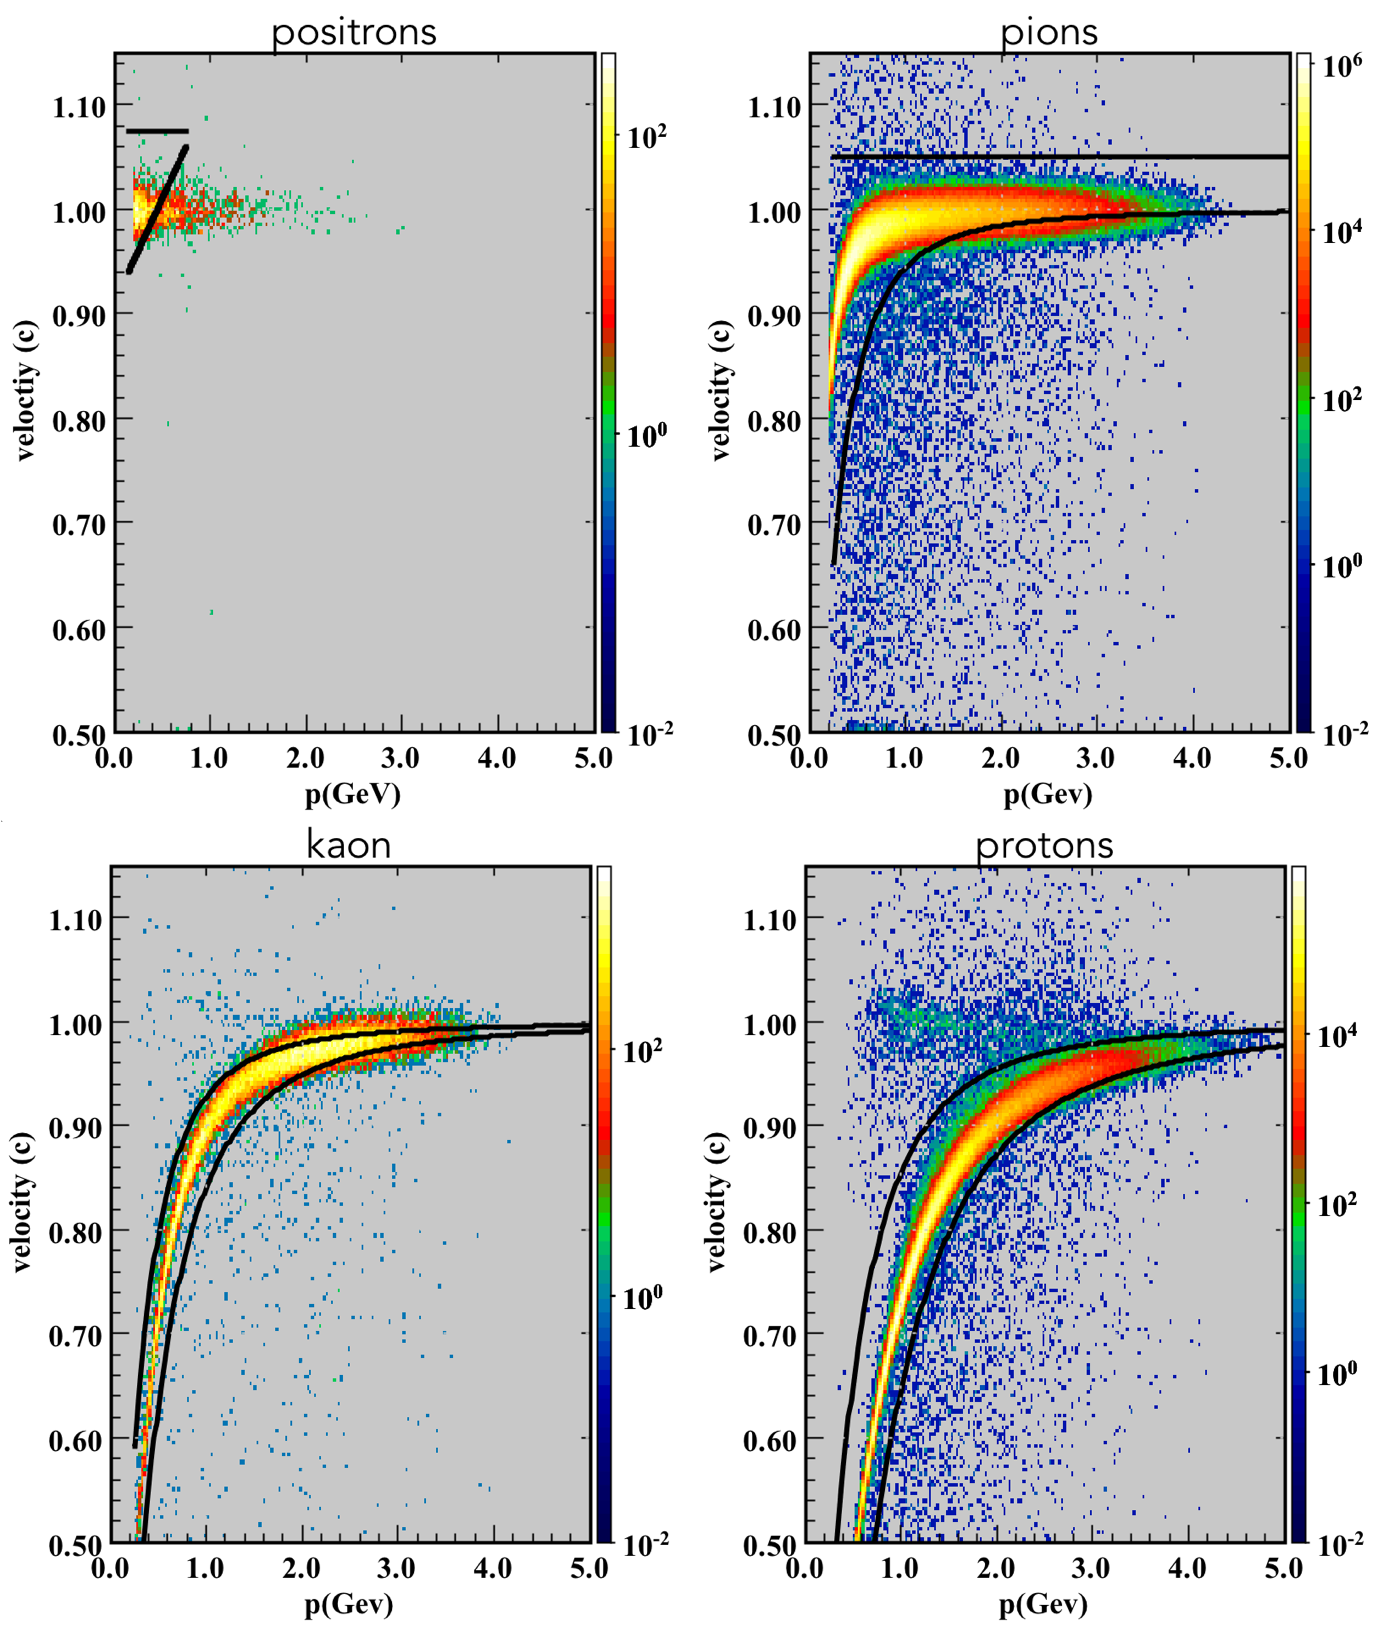
\includegraphics[width=\linewidth,height=70mm]{figures/bvp_grid.png}
\label{fig:bvp_grid}
\end{minipage}
\hfill
\begin{minipage}[c]{0.54\linewidth}
\vspace{-6mm}
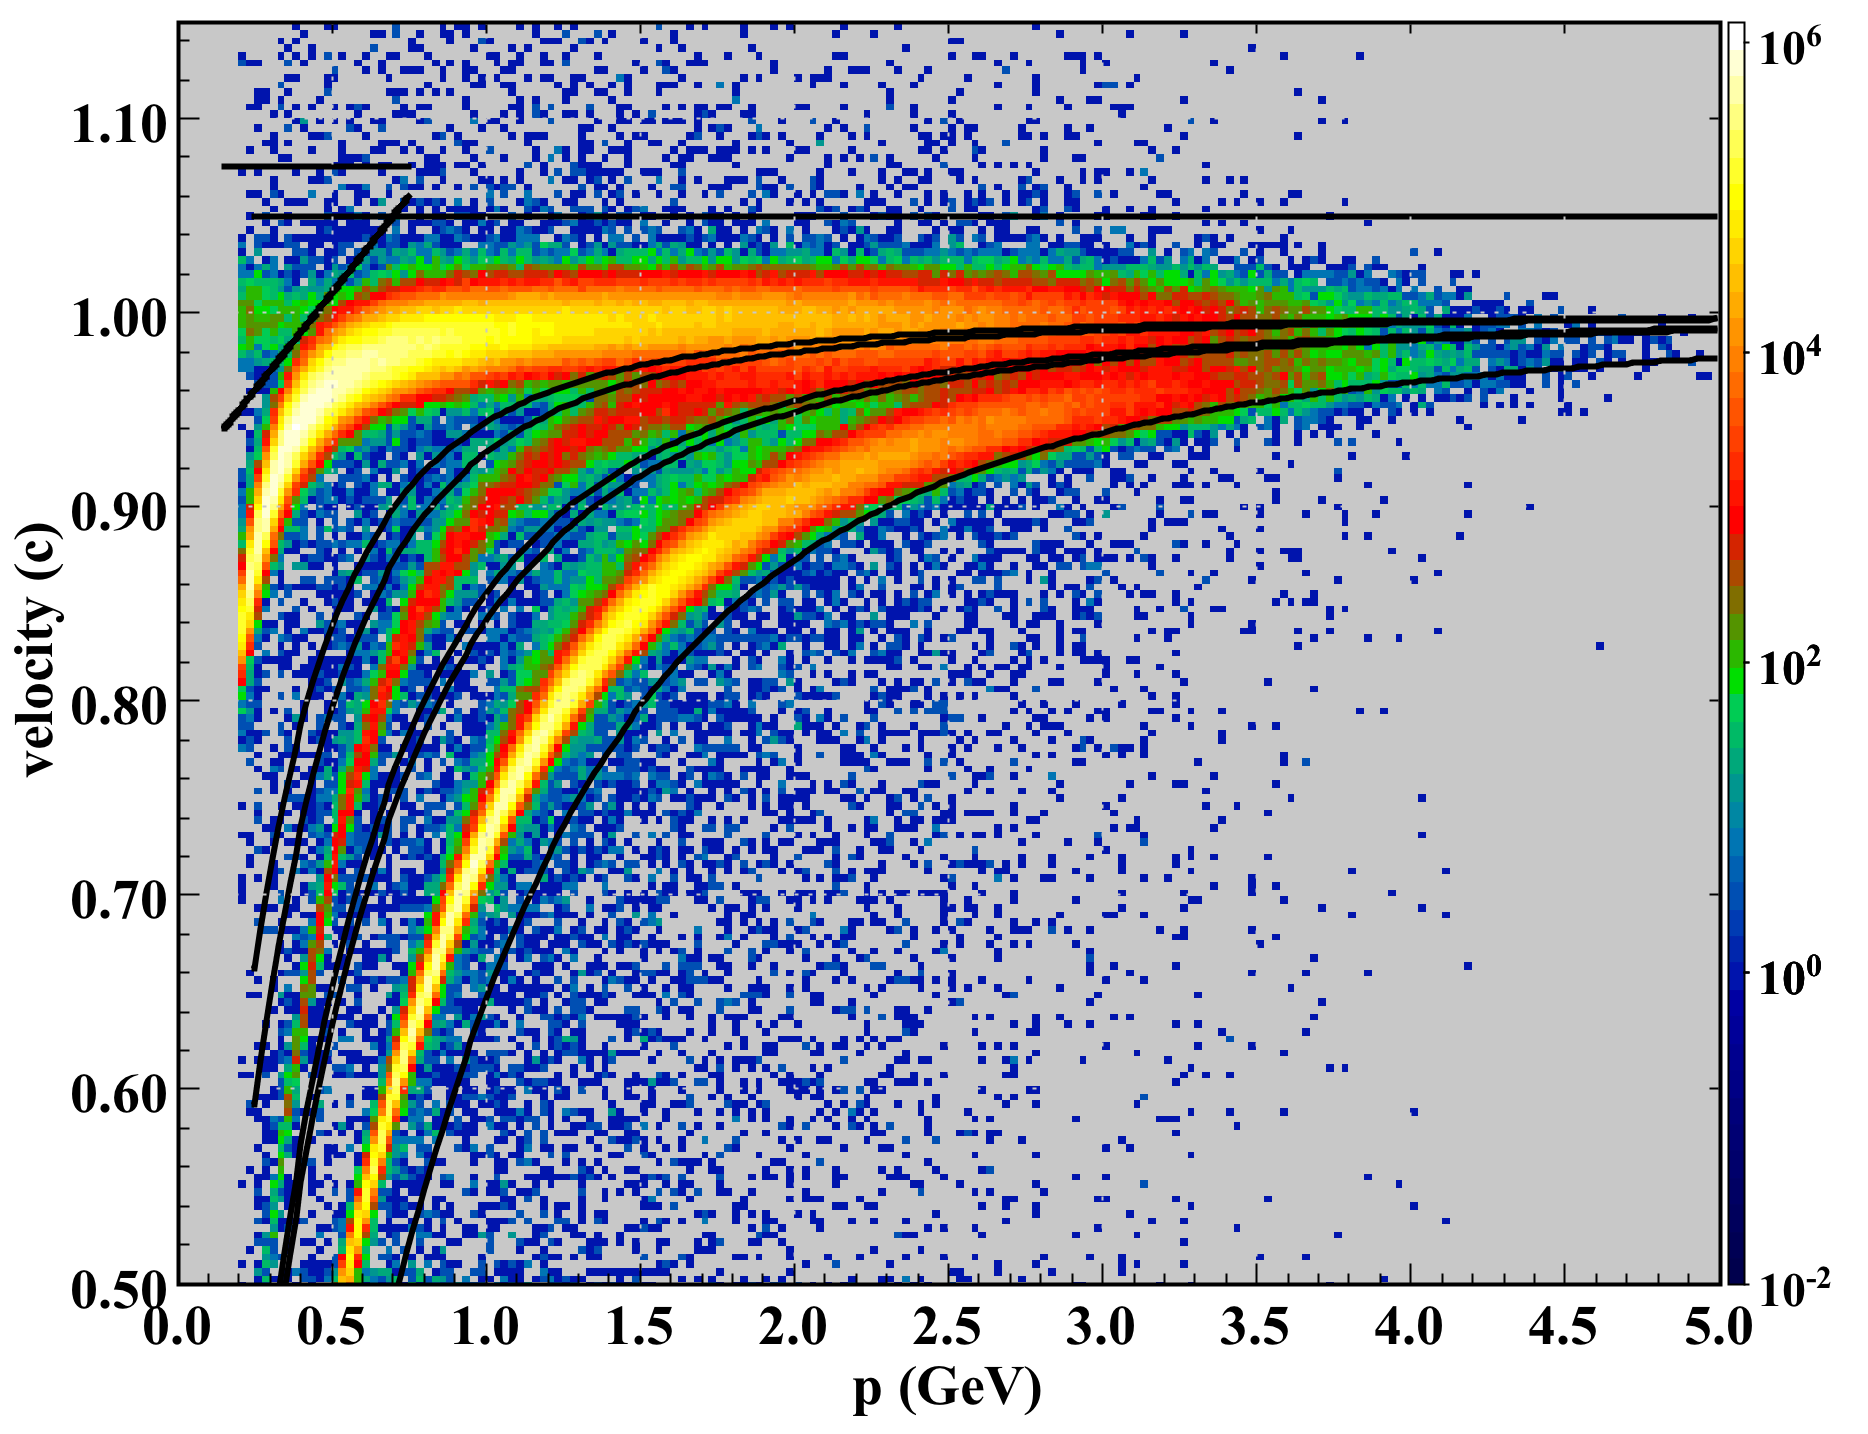
\includegraphics[width=\linewidth,height=55mm]{figures/bvp_all.png}
\vspace{-6mm}
\captionof{figure}{Left: $\beta$ vs p for each of the 4 particles studied. Right: $\beta$ vs p summed over all 4 particles. The black lines represent the upper and lower cuts.}
\label{fig:bvp_all}
\end{minipage}
\end{center}

\vspace{-5mm}
The second method studied used simulated data to create a multi-dimensional probability distribution for each particle type as a function of all 6 detector responses.
The distribution consisted of four six-dimensional histograms where the binning scheme was tuned to maximize efficiency and purity.

The third PID method used was machine learning, specifically a neural network.
Several topologies, activation functions, learning rates, and backpropagation algorithms were studied and compared.
}

%%%%%%%%%%%%%%%%%%%%%%%%%%%%%%%%%%%%%%%%%%%%%%%%%%%%%%%%%%%%%%%%%%%%%%%%%%%%%%
  \headerbox{Results}{name=results,column=2,below=methods,span=2}{
%%%%%%%%%%%%%%%%%%%%%%%%%%%%%%%%%%%%%%%%%%%%%%%%%%%%%%%%%%%%%%%%%%%%%%%%%%%%%%
\noindent{
Figure \ref{fig:rocs} shows the efficiency and purity of each particle sample for each of the three PID methods.
The multiple points come from adjusting various parameters to search for the optimal result.
Points closest to the top-right of the plot (100\% efficiency, 100\% purity) are considered best.
}
%
\begin{center}
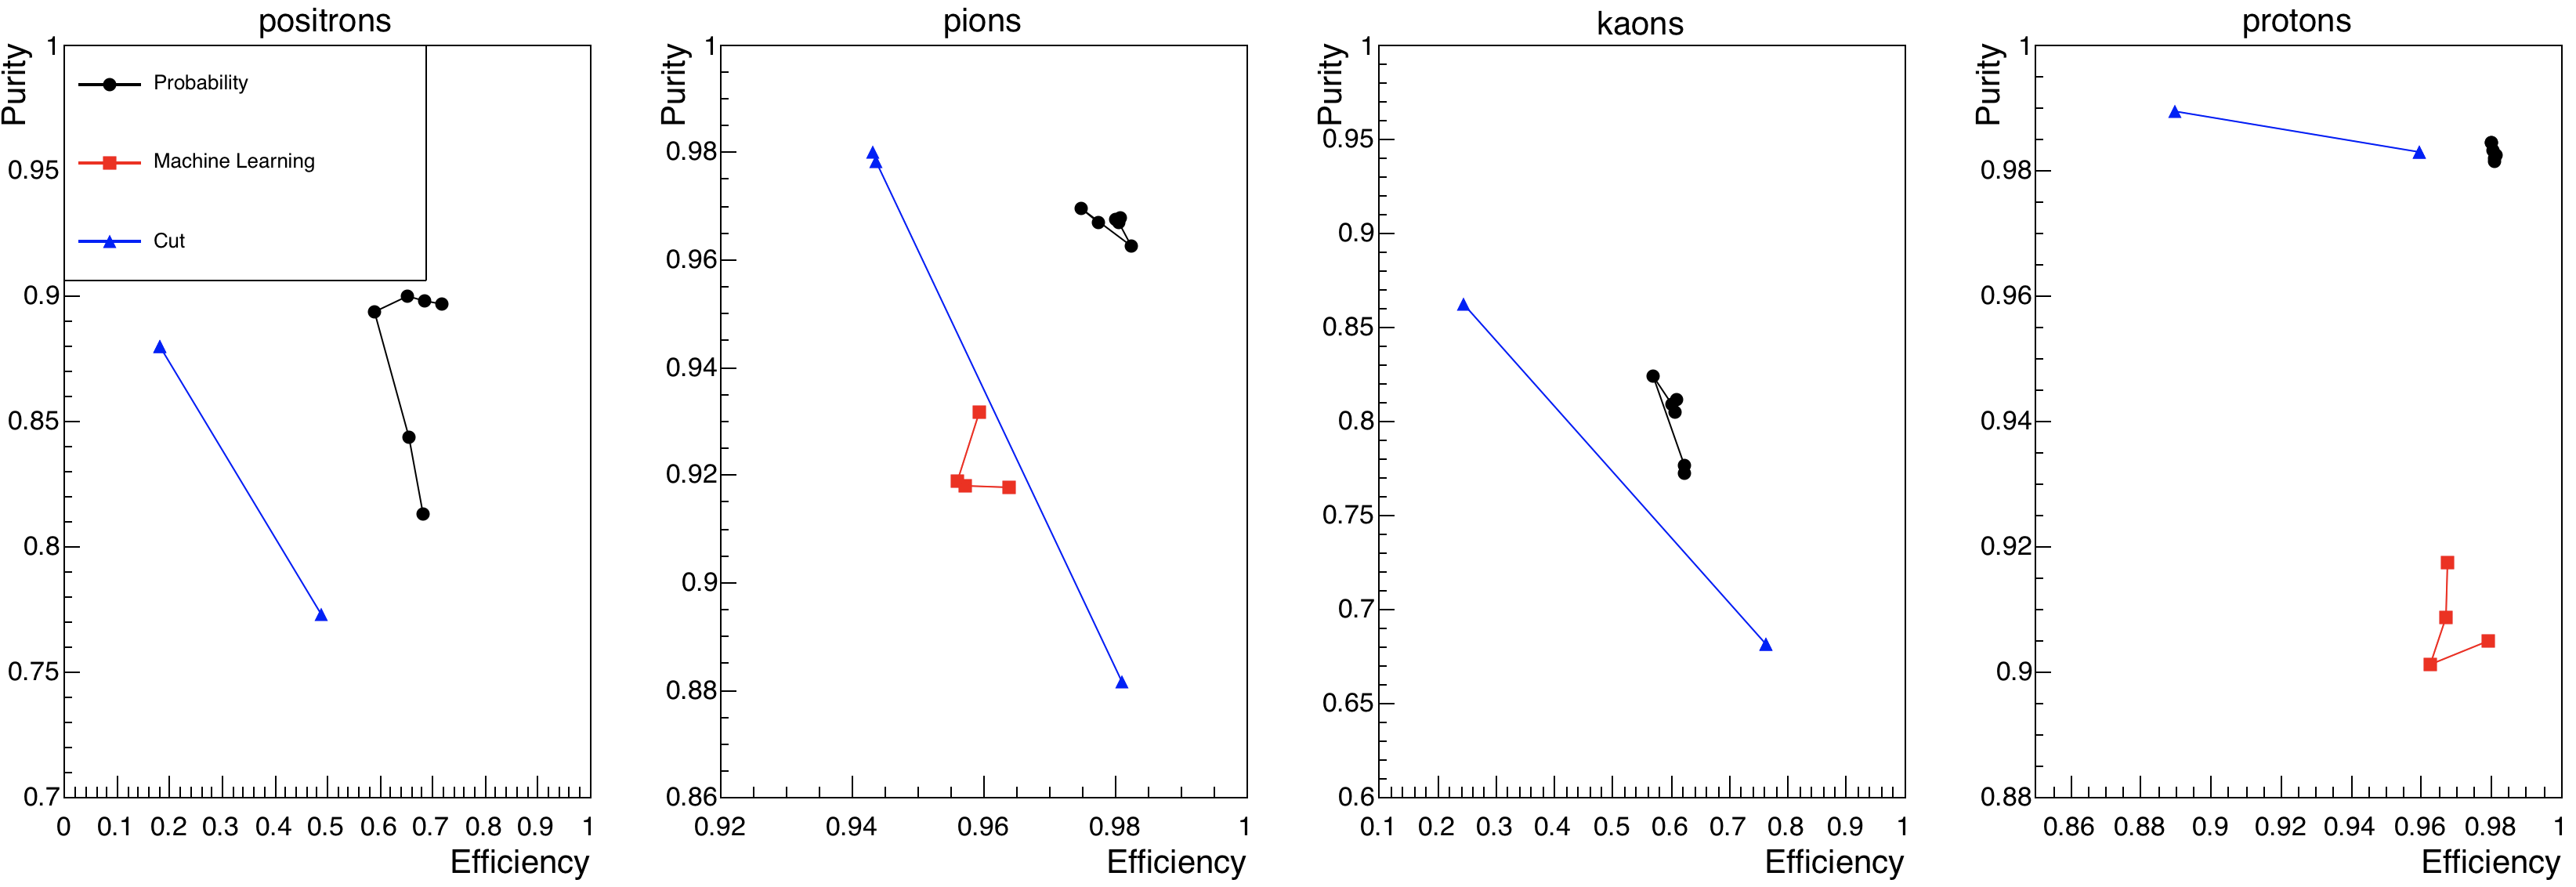
\includegraphics[width=\linewidth,height=52mm]{figures/rocs.png}
\captionof{figure}{Purity vs. efficiency curves for each particle sample and each PID method.}
\label{fig:rocs}
\end{center}
}

%%%%%%%%%%%%%%%%%%%%%%%%%%%%%%%%%%%%%%%%%%%%%%%%%%%%%%%%%%%%%%%%%%%%%%%%%%%%%%
  \headerbox{Conclusion and Discussion}{name=conclusion,column=0,below=introduction,span=2}{
%%%%%%%%%%%%%%%%%%%%%%%%%%%%%%%%%%%%%%%%%%%%%%%%%%%%%%%%%%%%%%%%%%%%%%%%%%%%%%
\noindent{
The probability method consistently gave the best results, however model dependence is a big concern that will be studied in the future.
For a first try, the machine learning results are promising, but better optimization of the algorithm is needed.
Model dependence is a concern here as well and further studies are needed; unsupervised learning will also be investigated in the future.
It appears likely that the best PID will come from a combination of all of these techniques; for example, the cut-based approach is very effective at low momenta, but the other two approaches perform better at high momenta.
}
}

%%%%%%%%%%%%%%%%%%%%%%%%%%%%%%%%%%%%%%%%%%%%%%%%%%%%%%%%%%%%%%%%%%%%%%%%%%%%%%
  \headerbox{References}{name=references,column=0,below=conclusion,span=2,bottomaligned=results}{
%%%%%%%%%%%%%%%%%%%%%%%%%%%%%%%%%%%%%%%%%%%%%%%%%%%%%%%%%%%%%%%%%%%%%%%%%%%%%%
{ \footnotesize
\noindent{$[1]$ Geant4 - A Simulation Toolkit, S. Agostinelli et al., Nucl. Instrum. Meth. A 506 (2003) 250-303}

\vspace{1mm}
\noindent{$[2]$ The CEBAF Large Acceptance Spectrometer (CLAS), The CLAS Collaboration, Nucl.Instrum.Meth. A503, 513 (2003)}

\noindent{$[3]$ Probing high-momentum protons and neutrons in neutron-rich nuclei, The CLAS Collaboration, Nature 560, 617–621 (2018)}
}

}


\end{poster}

\end{document}
